\label{section:results}

\begin{table*}[t!]
\centering
\begin{tabular}{c|c|c|c|c|c|c|c|c|c|c}
        &         & Num       & Lines     &        &        & Potential & Validated  &         & Inj Time \\
Name    & Version & Src Files & C code    & N(DUA) & N(ATP) & Bugs      & Bugs       & Yield   & (sec)  \\\hline
file    & 5.22    & 19        & 10809     & 631    & 114    & 17518     & 774        & 39.0\%  & 16         \\  %    files verified.  sloc recomputed
%eog    & 3.4.2   &           & 22997     &        &        &           &            &         &         \\ 
readelf & 2.25    & 12        & 21052     & 3849   & 266    & 276367    & 1064       & 53.4 \% & 354     \\  % time verified.  files verified. sloc recomputed
bash    & 4.3     & 143       & 98871     & 3832   & 604    & 447645    & 192        & 9.5\%   & 153     \\  % time verified.  
tshark  & 1.8.2   & 1272      & 2186252   & 9853   & 1037   & 1240777   & 354        & 15.3\%  & 542     \\
\end{tabular} 
\caption{LAVA Injection results for open source programs of various sizes.
For each, a single input file was used to perform a taint analysis with PANDA.
Various program and dynamic trace statistics are reported as well as DUA, attack point (ATP), and yield (fraction of injected bugs that result in a segmentation violation).}
\label{table:insertion-results}
\end{table*}

%We evaluated LAVA in three ways.
We evaluated LAVA in two ways.
First, we injected large numbers of bugs into four open source programs: file, readelf (from binutils), bash, and tshark (command-line verison of Wireshark). %, and eog (aka Eye of GNOME, an image viewer).
For each of these, we report various statistics with respect to both the target program and also LAVA's success at injecting bugs.
Second, we evaluated the distribution and realism of LAVA's bugs by proposing and computing various measures.
%Third, we randomly sampled 20 injected bugs for each of these programs and used these to measure detection rates for two commercial and two open source bug finders.

\subsection*{Counting Bugs}

Before we delve into the results, we must specify what it is we mean by an injected bug, and what makes two injected bugs distinct. Although there are many possible ways to define a bug, we choose a definition that best fits our target use case: two bugs should be considered different if an automated tool would have to reason about them differently. For our purposes, we define a bug as a unique pair $(DUA, attack point)$. Expanding this out, that means that the source file, line number, and variable name of the DUA, and the source file and line number of the attack point must be unique.

Some might object that this artificially inflates the count of bugs injected into the program, for example because it would consider two bugs distinct if they differ in where the file input becomes available to the program, even if the same file input bytes are used in both cases. But in fact these should be counted as different bugs: the data and control flow leading up to the point where the DUA occurs will be very different, and vulnerability discovery tools will have to reason differently about the two cases.

\subsection{Injection Experiments}
\label{sec:results:subsec:injection}

The results of injecting bugs into open source programs are summarized in Table~\ref{table:insertion-results}.
In this table, programs are ordered by size, in lines of C code, as measured by David Wheeler's \verb+sloccount+.
A single input was used with each program to measure taint and find injectable bugs.
The input to \verb+file+ and \verb+readelf+ was the program \verb+ls+.
The input to \verb+tshark+ was a 16K packet capture file from a site hosting a number of such examples.  % [ http://www.stearns.org/toolscd/current/pcapfile/README.ethereal-pcap.html ]
%The input to \verb+eog+ was ... 
The input to \verb+bash+ was a 124-line shell script written by the authors.
% TRL -- removed this since table was too big and I wanted to add bug inj time
%The number of sequential and unique basic blocks in the PANDA trace for each program are reported as N(BBs) and N(BBu).
$N(DUA)$ and $N(ATP)$ are the number of DUAs and attack points collected by the FIB analysis.
Note that, in order for a DUA or attack point to be counted, it must have been deemed viable for some bug, as described in Section~\ref{sec:mining}.
The columns \emph{Potential Bugs} and \emph{Validated Bugs} in Table~\ref{table:insertion-results} give the numbers of both potential bugs found by FIB, but also those verified to actually return exitcodes indicating a buffer overflow (-11 for segfault or -6 for heap corruption) when run against the modified input.
The penultimate column in the table is \emph{Yield} which is the fraction of potential bugs what were tested and determined to be actual buffer overflows.
The last column gives the time required to test a single potential bug injection for the target.


Exhaustive testing was not possible for several reasons.
Larger targets had larger numbers of potential bugs and take longer to test; for example, \verb+tshark+ has over a million bugs and took almost 10 minutes to test.
This is because testing requires not only injecting a small amount of code to add the bug, but also recompiling and running the resulting program.
For many targets, we found the build to be subtly broken so that a \verb+make clean+ was necessary to pick up the bug injection reliably, which further increased testing time.
Instead, we attempted to validate 2000 potential bugs chosen uniformly at random.

As the injected bug is designed to be triggered only if a particular set of four bytes in the input is set to a magic value, we tested with both the original input and with the modified one that contained the trigger. 
We did not encounter any situation in which the original input triggered a crash.

\begin{table}[b]
\centering
\begin{tabular}{l|l|l|l|l} 
       & \multicolumn{3}{c}{$mLIV$} &  \\  
$mTCN$ &         $[0,10)$ & $[10,100)$ & $[100,1000)$ & $[1000,+\inf]$ \\  \hline 
$[0,10)$ &       51.9\%   & 22.9\%     & 17.4\%       & 11.9\%          \\
$[10,100)$ &     --       & 0          & 0            & 0     \\
$[100,+\inf]$ &  --       & --         & --           & 0     \\ 
\end{tabular}
\caption{Yield as a function of both $mLIV$ and $mTCN$.  
Yield is highest for DUAs with low values for both of these measures, i.e., that are both a relatively uncomplicated function of input bytes and also that derive from input bytes involved in deciding fewer branches.
Cells for which there were no samples are indicated with the contents '--'.}
\label{table:yield-breakdown}
\end{table}

Yield varies considerably from less than 10\% to over 50\%.
To understand this better, we investigated the relationship between our two taint-based measures and yield.
For each DUA used to inject a bug, we determined $mTCN$, the maximum TCN for any of its bytes and $mLIV$, the maximum liveness for any label in any taint label set associated with one of its bytes.  
More informally, $mTCN$ represents how complicated a function of the input bytes a DUA is, and $mLIV$ is a measure of how much the control flow of a program is influenced by the input bytes that determine a DUA.
Table~\ref{table:yield-breakdown} is a two-dimensional histogram with the bins for $mTCN$ intervals along the vertical axis and bins for $mLIV$ along the horizontal axis.
The top-left cell of this table represents all bug injections for which $mTCN<10$ and $mLIV<10$, and the bottom-right cell is all those for which $mTCN>=1000$ and $mLIV>=1000$.
Recall that when  $mTCN=mLIV=0$, the DUA is not only a direct copy of input bytes, but those input bytes have also not been observed to be used in deciding any program branches. 
As either $mTCN$ or $mLIV$ increase, yield deteriorates.  
However, we were surprised to observe that $mLIV$ values of over 1000 still gave yield in the 10\% range.

\subsection{Bug Distribution}

It would appear as though LAVA can inject a very large number of bugs.  
If we extrapolate from yield numbers in Table~\ref{table:insertion-results}, we estimate there would be almost 400,000 real bugs if all were tested.

\noindent
But how well distributed is this set of bugs? 
For programs like \verb+file+ and \verb+bash+, between 11 and 44 source files  are involved in a potential bug.
In this case, the bugs appear to be fairly well distributed, as those numbers represent 58\% and 31\% of the total for each, respectively.
On the other hand, \verb+readelf+ and \verb+tshark+ fare worse, with only 2 and 122 source files found to involve a potential bug for each (16.7\% and 9.6\% of source files).
For \verb+tshark+, much of the code for which is devoted to parsing esoteric network protocols, coverage is probably the issue since we use only a single input.
Similiary, we only use a single hand-written script with \verb+bash+, with little attempt to cover a majority of language features.
We are unsure why so few of the source files in \verb+readelf+ involve a potential bug.
 

\subsection{Bug Realism}

\todo[inline]{Ricky: I think it would be particularly convincing to have a "case study" of an actual CVE that exhibits data flow properties similar to the kind of bug LAVA injects.  Or maybe a bug that adds unchecked tainted data to a pointer.} 

\begin{figure}
\centering
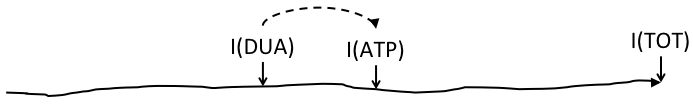
\includegraphics[width=3in]{trace-dua-atp.png}
\caption{A cartoon representing an entire program trace, annotated with instruction count at which DUA is siphoned off to be used, $I(DUA)$, attack point where it is used, $I(ATP)$, and total number of instructions in trace, $I(TOT)$.}
\label{fig:dua-atp-trace}
\end{figure}

The intended use of the bugs created by this system is as ground truth for development and evaluation of vulnerability discovery tools and techniques. 
Thus, it is crucial that they be realistic in some sense.  
Realism is, however, difficult to assess.

Because this work is, to our knowledge, the first to consider the problem of fully automated bug injection, we are not able to make use of any standard measures for bug realism.
Instead, we devised our own measures, focusing on features such as how well distributed the malformed data input and trigger points were in the program's execution, as well as how much of the original behavior of the program was preserved.

We examined three aspects of our injected bugs as measures of realism. 
The first two are DUA and attack point position within the program trace, which are depicted in Figure~\ref{fig:dua-atp-trace}.
That is, we determined the fraction of trace instructions executed at the point the DUA is siphoned off and at the point it is used to attack the program by corrupting an internal program value.
\todo[inline]{Ricky: what is the other "measures of realism?"  The "portion of hte trace between I(DUA) and I(ATP)? I(DUA)/I(ATP)? I(TOT)?} 

Histograms for these two quantities, $I(DUA)$ and $I(ATP)$, are provided in Figures~\ref{fig:dua-hist} and~\ref{fig:atp-hist}, where counts are for all potential bugs in the LAVA database for all five open source programs. 
DUAs and attack points are clearly available at all points during the trace, although there appear to be more at the beginning and end.
This is important, since bugs created using these DUAs have entirely realistic control and data-flow all the way up to $I(DUA)$.
Therefore, vulnerability discovery tools will have to reason correctly about all of the program up to $I(DUA)$ in order to correctly diagnose the bug.

The portion of the trace \emph{between} the $I(DUA)$ and $I(ATP)$ is of particular interest since LAVA currently makes data flow between DUA and attack point via a pair of function calls.
Thus, it might be argued that this is an unrealistic portion of the trace in terms of data flow.
The quantity $I(DUA)/I(ATP)$ will be close to 1 for injected bugs that minimize this source of unrealism.
This would correspond to the worked example in Figure~\ref{fig:worked-example}; the DUA is still in scope when, a few lines later in the same function, it can be used to corrupt a pointer.
No abnormal data flow is required.
The histogram in Figure~\ref{fig:rdf-hist} quantifies this effect for all potential LAVA bugs, and it is clear that a large fraction have $I(DUA)/I(ATP) \approx 1$, and are therefore highly realistic.

\begin{figure}
\centering
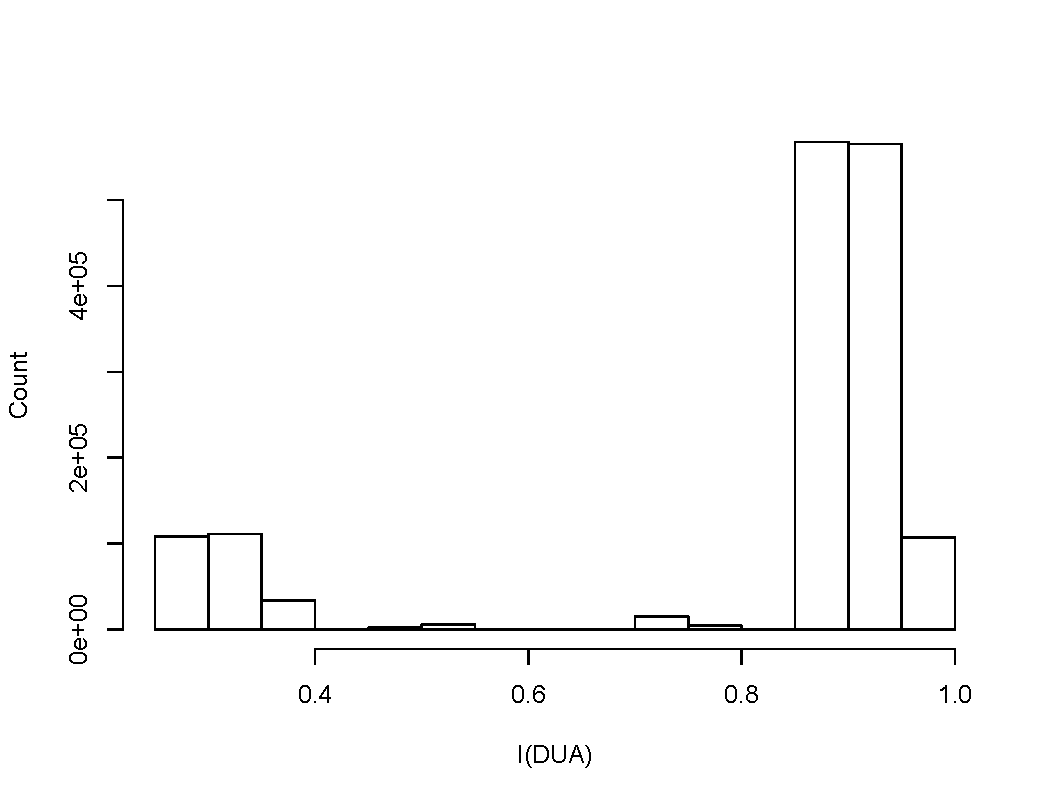
\includegraphics[width=3in]{dua.pdf}
\caption{Normalized DUA trace location}
\label{fig:dua-hist}
\end{figure}

\begin{figure}
\centering
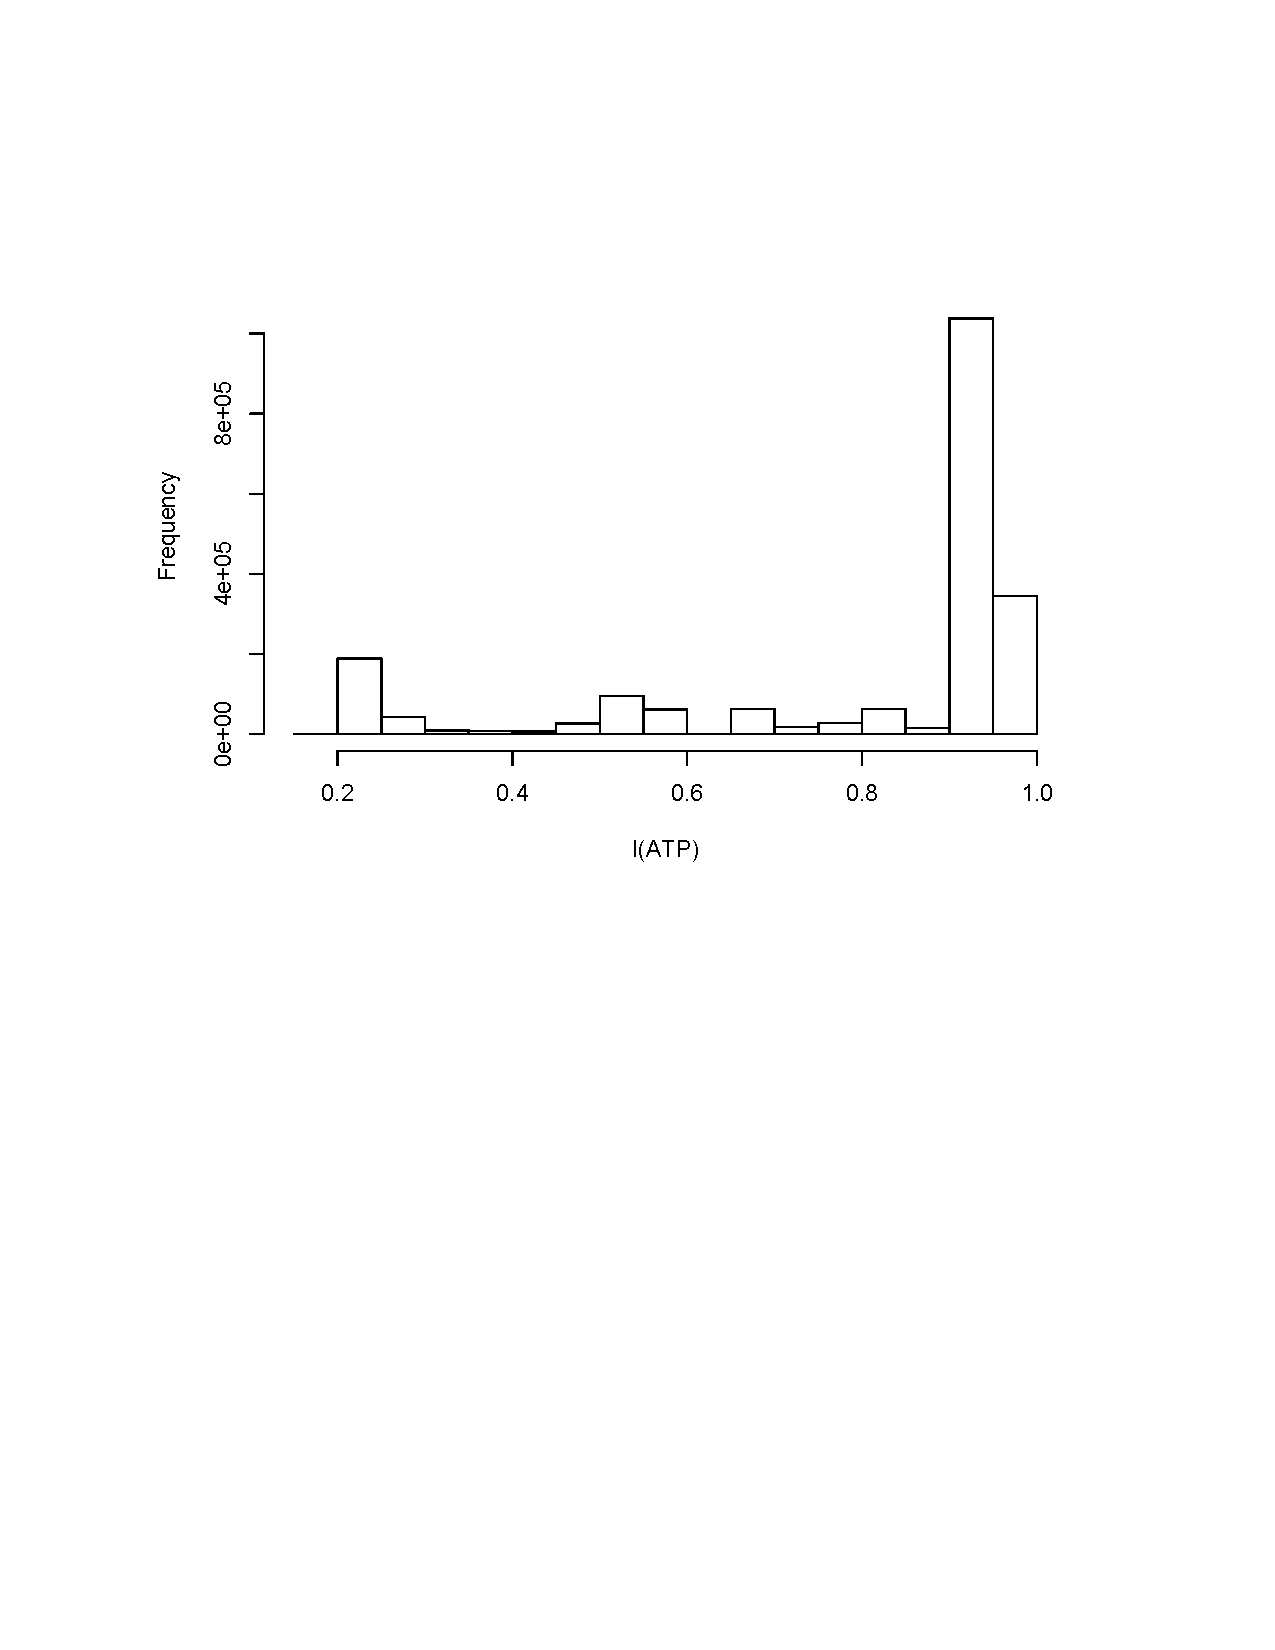
\includegraphics[width=3in]{atp.pdf}
\caption{Normalized ATP trace location}
\label{fig:atp-hist}
\end{figure}

\begin{figure}
\centering
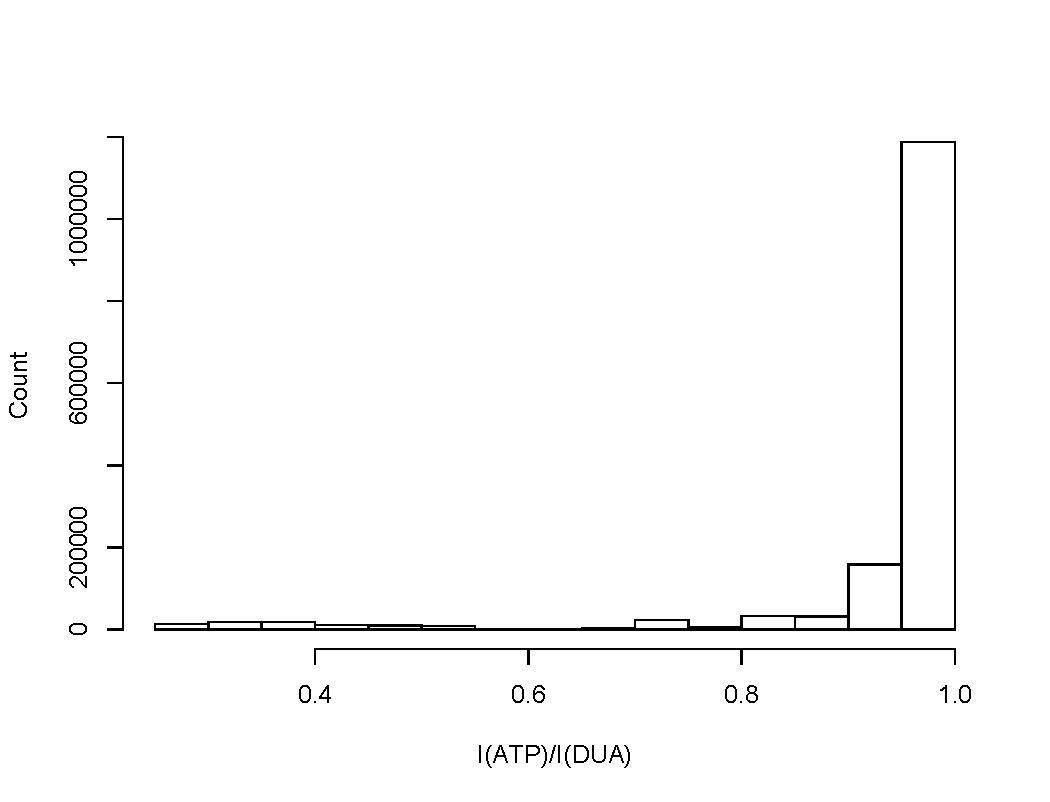
\includegraphics[width=3in]{rdf.pdf}
\caption{Fraction of trace with perfectly normal or realistic data flow, $I(DUA)/I(ATP)$}
\label{fig:rdf-hist}
\end{figure}




\subsection{Vulnerability Discovery Tool Evaluation}
We ran four vulnerability discovery tools on LAVA-injected bugs to investigate their use in evaluation.
\begin{enumerate}
\item Open-source fuzzer (referred to as FUZZER)
\item Commercial static analyzers (referred to as CSA) % 1 and CSA2)
\item Symbolic execution + SAT solver system (referred to as SES)
\end{enumerate}
The tools were selected to span the range of approaches employed by automated bug finders, constrained by availability.
FUZZER and SESAT are both state-of-the-art, high-profile tools. 
%CSA1 and CSA2, both closed-source, appear to use quite different approaches according to their advertising literature.
For every tool, we expended significant effort to ensure that we were using tools correctly.
This means carefully reading all documentation, blog posts, and email lists.
Additionally, we constructed tiny example buggy programs and used them to verify that we were able to use each tool to find them.  
For some tools we had to resort to reading source code in order to determine the correct command-line incantations to employ. 
In no case did we contact tool authors or companies for guidance in tool use, as this seemed likely to bias results.

Note that the names of tools under evaluation are being withheld in reporting results.
Careful evaluation is a large and important job, and we would not want to give it short shrift, either in terms of careful setup and use of tools, or in presenting and discussing results.
Our intent, here, is to determine if LAVA bugs \emph{can be used} to evaluate a bug finding system. 
It is our expectation that, in future work either by ourselves or others, full and careful evaluation of real, named tools will be performed using LAVA.
Additionally, it is our plan and hope that LAVA bugs can be made available for self-evaluation and hill climbing.

The first corpus was created using the \verb+file+ target, the smallest of those into which we have injected bugs.
LAVA was used to inject 69 buffer overflow bugs.
Each bug was inserted into a different branch of the source, and came with a fuzzed version of the input that was verified to trigger either a segfault or heap corruption.  
Two types of buffer overflows were injected each of which makes use of a single 4-byte DUA to trigger and control the overflow.
\begin{enumerate}
\item \emph{Knob-and-trigger}.  In this type of bug, two bytes of the DUA are to test against a magic value to determine if the overflow will happen, while the other two bytes of the DUA determine how much to overflow.   Thus, these bugs manifest if a 2-byte unsigned integer is a magic value and some other 2-byte unsigned integer determines the extent of the overflow. 
\item \emph{Range}.  These bugs trigger if the magic value is in some range, but also use the magic value to determine how much to overflow.
The magic value is a 4-byte unsigned integer and the range varies.
\end{enumerate}
The results of this evaluation are summarized in Table~\ref{table:eval1-file}
Five different ranges were employed: $1, 128, 16384, 2097152, 268435456$. 
Unfortunately, SES was unable to analyze \verb+file+ due to unsupported library calls.
Thus, we only have results for FUZZER and CSA.
We examined all of the output from both tools.  
CSA found none of the LAVA bugs, but ran in a very short time.  
FUZZER ran for one hour on each bug and found 7\% of those with a range of 2097152 and 58\% of those with a range size of 268435456.

These results seem to accord with both how these LAVA bugs work and also what we know about how these two tools work.
CSA is a code scanner which looks for dodgy patterns in source code.
It is unlikely to be performing a deep and detailed analysis as it runs so quickly.
FUZZER uses the program largely as a black box, randomizing individual bytes, and using coverage to guide exploration.  
Bugs that trigger if and only if a four-byte extent in the input is set to a magic value are unlikely to be discovered in this way.
Given time, FUZZER finds bugs that trigger for ranges of a million or more bytes. 
For many of these LAVA bugs, when the range is so large, discovery is possible by simply fuzzing every byte in the input a few times.  
These bugs may, in fact, be trivially discoverable with a regression suite for a program like \verb+file+ that accepts arbitrary file input\footnote{In principle, anyway. In practice file's test suite consists of just 3 tests, none of which trigger our injected bugs.}.

Note that having each bug on a separate branch means that, for each run of a bug finding tool, only one bug is available for discovery at a time.  
This is one kind of evaluation, but it seems to disadvantage tools like FUZZER and SES, which appear to be designed to work for a long time (10s of hours) on a single program that includes perhaps a number of bugs. 
To address this issue and also to allow all tools to be evaluated on a single program, we arranged to have LAVA inject more than one bug into the source code.
We chose four programs from the \verb+coreutils+ suite after first determining that all four tools were capable of analyzing it.
LAVA injected 52 bugs into \verb+who+.  

We chose an open source fuzzer, two Commericial Static Analyzers (CSAs), and a Symbolic Execution and SAT Solver (SES) because they represented three unique approaches to vulnerability discovery.
Our corpora was a collection of 69 modifications of the program \verb+file+.
Each modification represented one of six different bug types and a randomly selected $Bug ID$.
All the tools were run on the same system, a x64 Debian 7 server with 16 cores at 3.50 GHz and 365 gB of \uppercase{ram}.
The tools were run to completion except in the case of the fuzzer where a wall time of 1 hour was given.
The evaluation results are summarized in Table~\ref{table:eval-results}. 

\begin{table}[h]
\centering
\begin{tabular}{l|l|l|l|l|l|l} 
$Tool Type$ &                     \multicolumn{6}{|c}{$Bug Type$}                           \\  \hline  
            &                     \multicolumn{5}{|c|}{$Range Bug$}               & $KT$    \\   
            &    1       & $2^7$       & $2^{14}$     & $2^{21}$   & $2^{28}$     & 1   \\  \hline 
$Fuzzer$    &    0       & 0           & 0            & 7\%        & 58\%         & 0         \\
$CSA_1$       &    0       & 0           & 0            & 0          & 0            & 0         \\
$SES$       &    0       & 0           & 0            & 0          & 0            & 0         \\
\end{tabular}
\caption{Percentage of bugs found as a function of $Bug Type$ and $Tool Type$.  The most effective vulnerability finding tool proved to be the open source fuzzer.  However, it was only able to find bugs that had an enormous range of possible inputs to trigger the bug.}
\label{table:tool-eval-results}
\end{table}

\begin{table}[h]
\centering
\begin{tabular}{l|c|c|c|c|c} 
\multirow{2}{*}{Tool Name} & \multirow{2}{*}{Total Bugs} & \multicolumn{4}{c}{Unique Bugs Found} \\
              &            & $Fuzzer$    & $CSA_1$      & $SES$      & $Combined$ \\ \hline 
\verb+uniq+   &    28      & 7           & 0            & 0          & 0               \\
\verb+base64+ &    44      & 7           & 0            & 0          & 0               \\
\verb+md5sum+ &    57      & 2           & 0            & 0          & 0               \\
\verb+who+    &    2286    & 0           & 0            & 0          & 0               \\
Total         &    2415    & 16          & 0            & 0          & 0               \\
\end{tabular}
\caption{Bugs found in selected GNU coreutils programs by each tool type.}
\label{table:tool-eval-results-coreutils}
\end{table}

We also evalued a second commercial static analyzer, referred to in this text as $CSA_2$. Because we were only allowed a limited number of analysis runs, we opted to create a single version of \verb+who+ from the GNU coreutils that contained 60 injected, verified bugs. This was fed to $CSA_2$, generating 117 alerts; we then went through its alerts by hand to see which ones referenced our injected bugs.

Of the 117 alerts, 17 referred to code we had injected into \verb+who+. We did not investigate the other 100 further; presumably these are some mix of true and false positives in the original source code to \verb+who+. The 17 that were specific to our injected bugs were examined in more detail. Fourteen were found to be essentially false positives: they referred to innocuous artifacts of the injection process. For example, to guard against introducing pointer errors, we emit code like \verb+if(p) { ... }+; however, the static analysis software took this as proof that \verb+p+ might be NULL, and then warned us that it was dereferenced elsewhere before the NULL check. After discounting such artifacts, we found that $CSA_2$ correctly identified three of our injected bugs, labeling them all as ``Out-of-bounds access''.

\subsection*{Discussion}
